\section{The Equipment in Use}\label{sec:hardware}
The aim of this chapter is to document the building of the speaker stand for measuring the polar response of the speaker array. The requirement for the stand is that it is able to be fixed to the turntable. That the stand is able to support the rather heavy loudspeakers and therefore a metal speaker stand construction has been chosen.  The construction is built such that the speaker is raised at least \SI{1}{\meter} from the turntable, to avoid reflections. A drawing of the turntable is illustrates the usable mounting points in \autoref{fig:turn_table}.


 \begin{figure}[H]
	\centering
	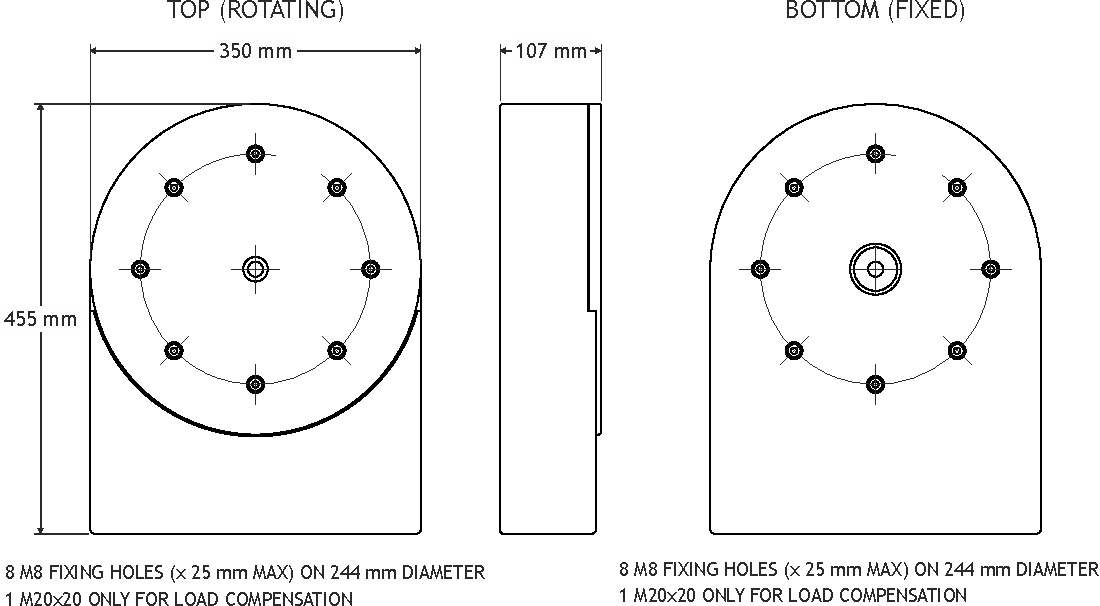
\includegraphics[width=1\textwidth]{ET250-3D_drawing}
	\caption{A drawing of the Outline turntable ET 250-3D, source: \citep{ET250-3D}}
		\label{fig:turn_table}
\end{figure}



The drawing of the turntable in \autoref{fig:turn_table} shows that the turning part of the turntable has a diameter of \SI{350}{\milli\meter}. The speaker construction shall at least have a diameter of \SI{1.1}{\meter}, such that loudspeakers can be mounted in a way, that separates the acoustical centers by \SI{400}{\milli\meter}. To achieve more stability for the speaker stand, the rotating part of the turntable is extended by a circular wood plate with a diameter of \SI{800}{\milli\meter}. The circular plate is bolted to the eight M8 screw holes seen in \autoref{fig:turn_table}. \\
The profile of the speaker stand has to be as small as possible to avoid reflection from construction, but it shall be rigid enough to hold the speaker in a constant position relative to eachother. Therefore it has been chosen to use squared metal pipe (box section) for the construction.  Because the speaker cabinets are placed close to each other, they may inflict the sound field, therefore some compensation by altering the loudspeaker positions is required. Therefore the placement of the loudspeakers has to be adjustable. The squared metal pipe is therefore divided intro a bottom part and three stand parts. To make the adjustable features possible, the bottom part is build out of \SI{45}{\milli\meter} box section and the stand part is built of \SI{40}{\milli\meter} box section. This enables the stand to be slid intro the bottom part. To achieve higher stability, the outer \SI{200}{\milli\meter} of bottom part is cut out as a ``u'' shape as visualized in \autoref{fig:botom_u}

 \begin{figure}[H]
	\centering
	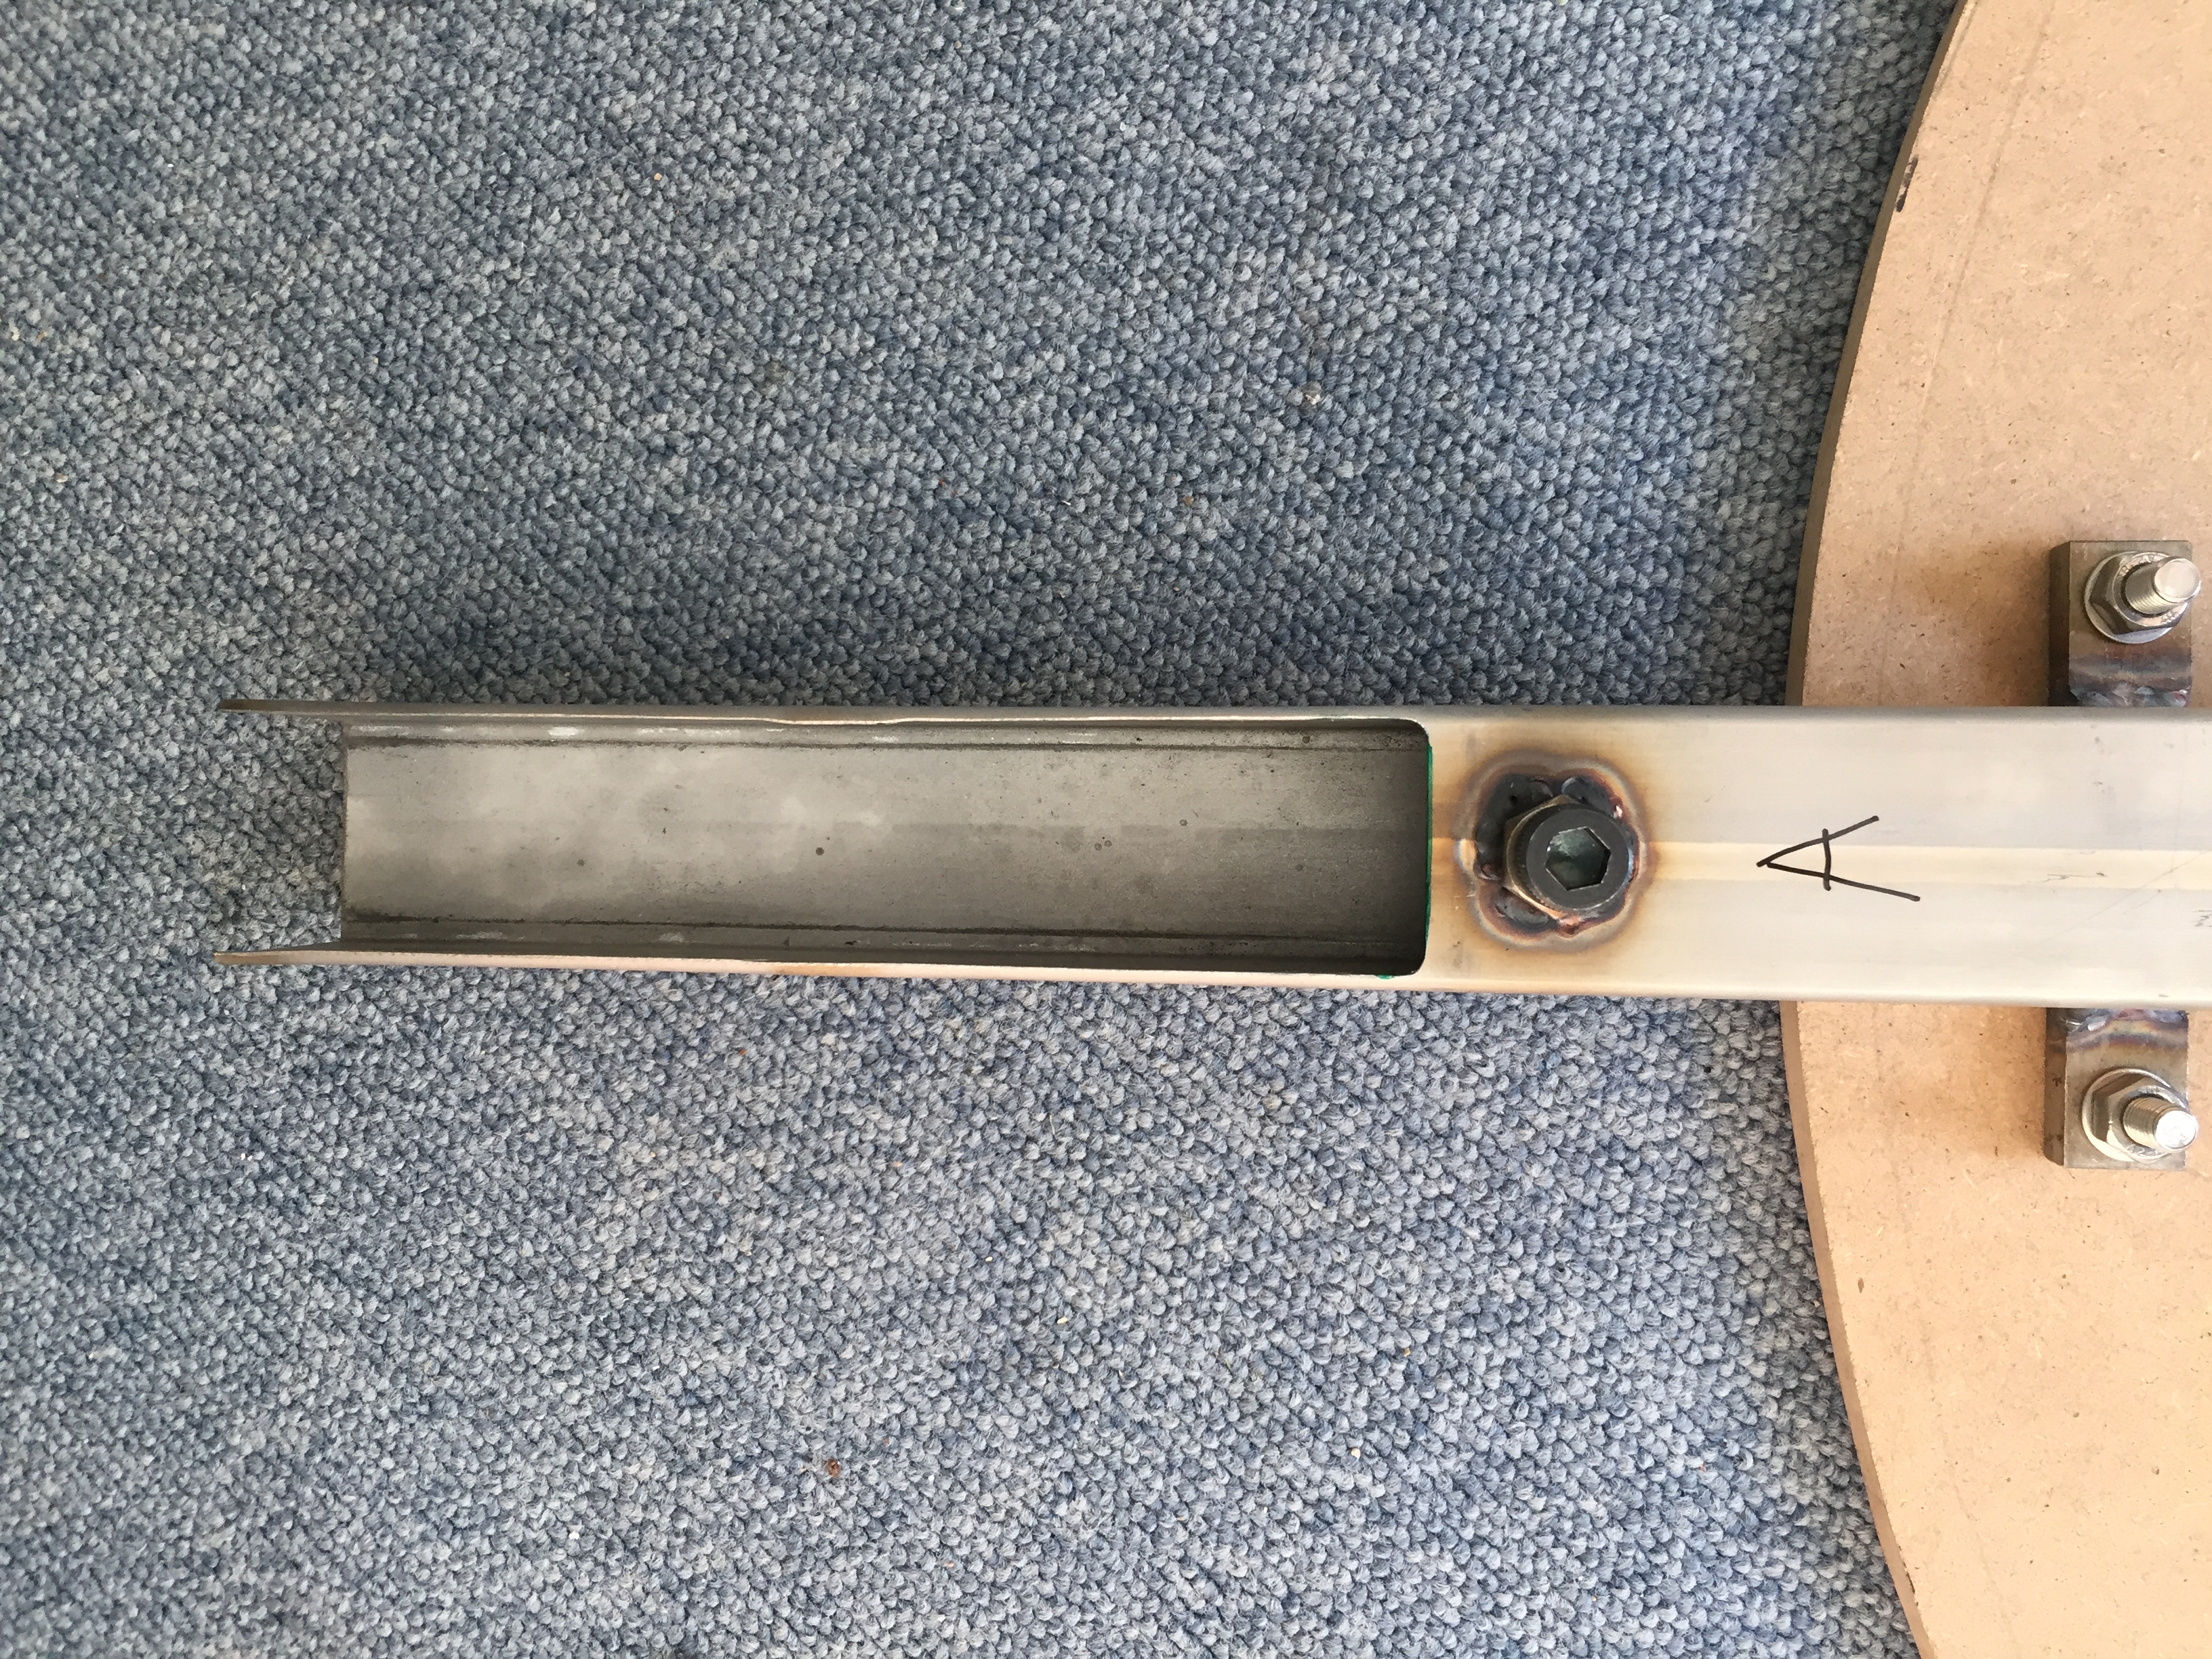
\includegraphics[width=1\textwidth]{bottom_u}
	\caption{The bottom part of the speaker stand with the u cut}
		\label{fig:botom_u}
\end{figure}

The acoustic centers of the loudspeakers have to be placed in a triangular shape, where it has been chosen to make the centroid as the array center (see \autoref{sec:genetic_implememtation}, \autoref{ax:directional_3}). This placement leads to a weight bias towards the direction, where the back speaker is placed, rotational axis of the turntable. Therefore a small plate is mounted in the front, such that it is possible to mount a counterweight to the speaker stand. The constructional drawing of the bottom part of the speaker stand is given in \autoref{fig:botom_final}

\begin{figure}[H]
	\centering
	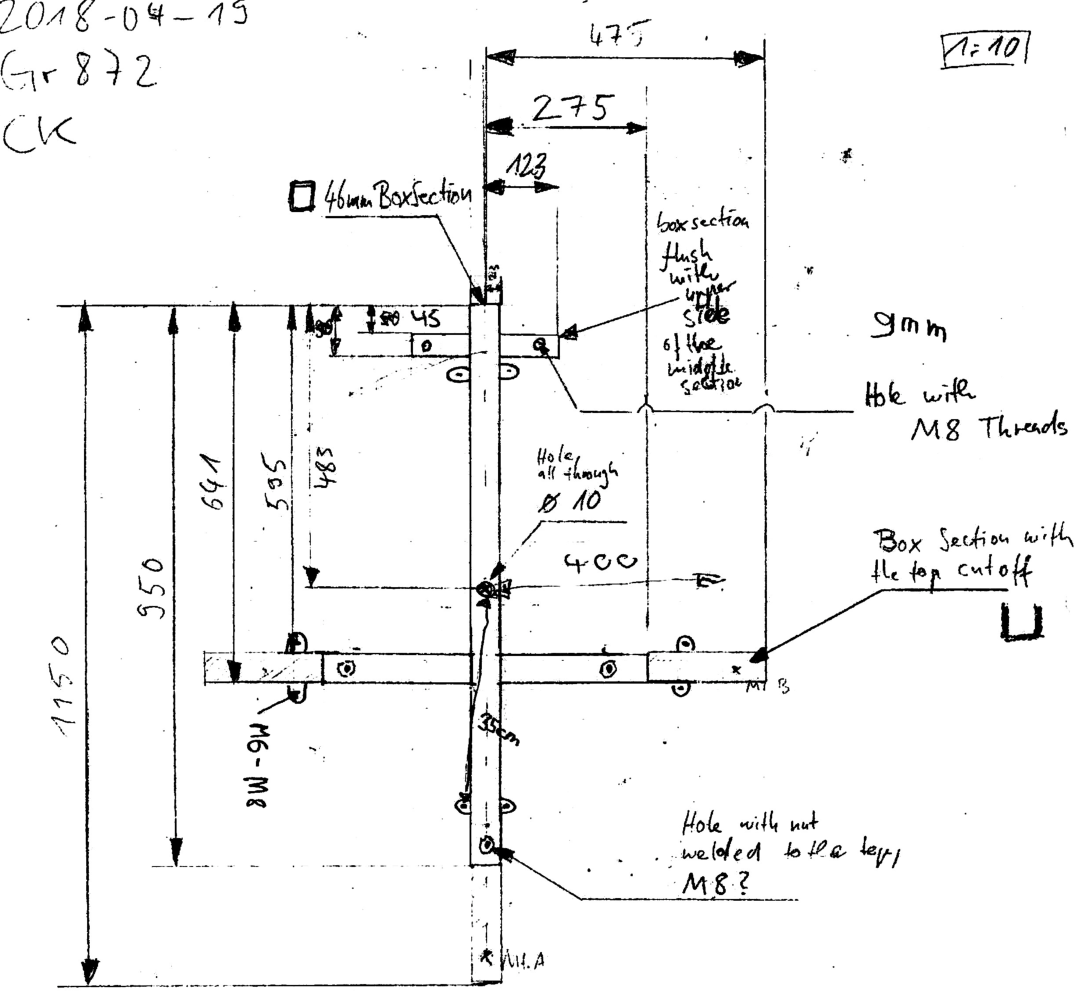
\includegraphics[width=1\textwidth]{bottom_final.pdf}
	\caption{Constructional drawing of array mounting system, bottom part.}
		\label{fig:botom_final}
\end{figure}

The corresponding loudspeaker stands are made in a ``L'' shape, where the horizontal part of the ``L'' can be slid into the formerly mentioned bottom part and the vertical part is used as the height extender, where the speaker is on top. The adjustability of the speaker stands also means, that before any measurement can be conducted, the loudspeaker positions have to be carefully tuned to the desired specifications. The following \autoref{fig:the_setup} shows the full speaker setup in the anechoic chamber at \gls{aau}.

  \begin{figure}[H]
	\centering
	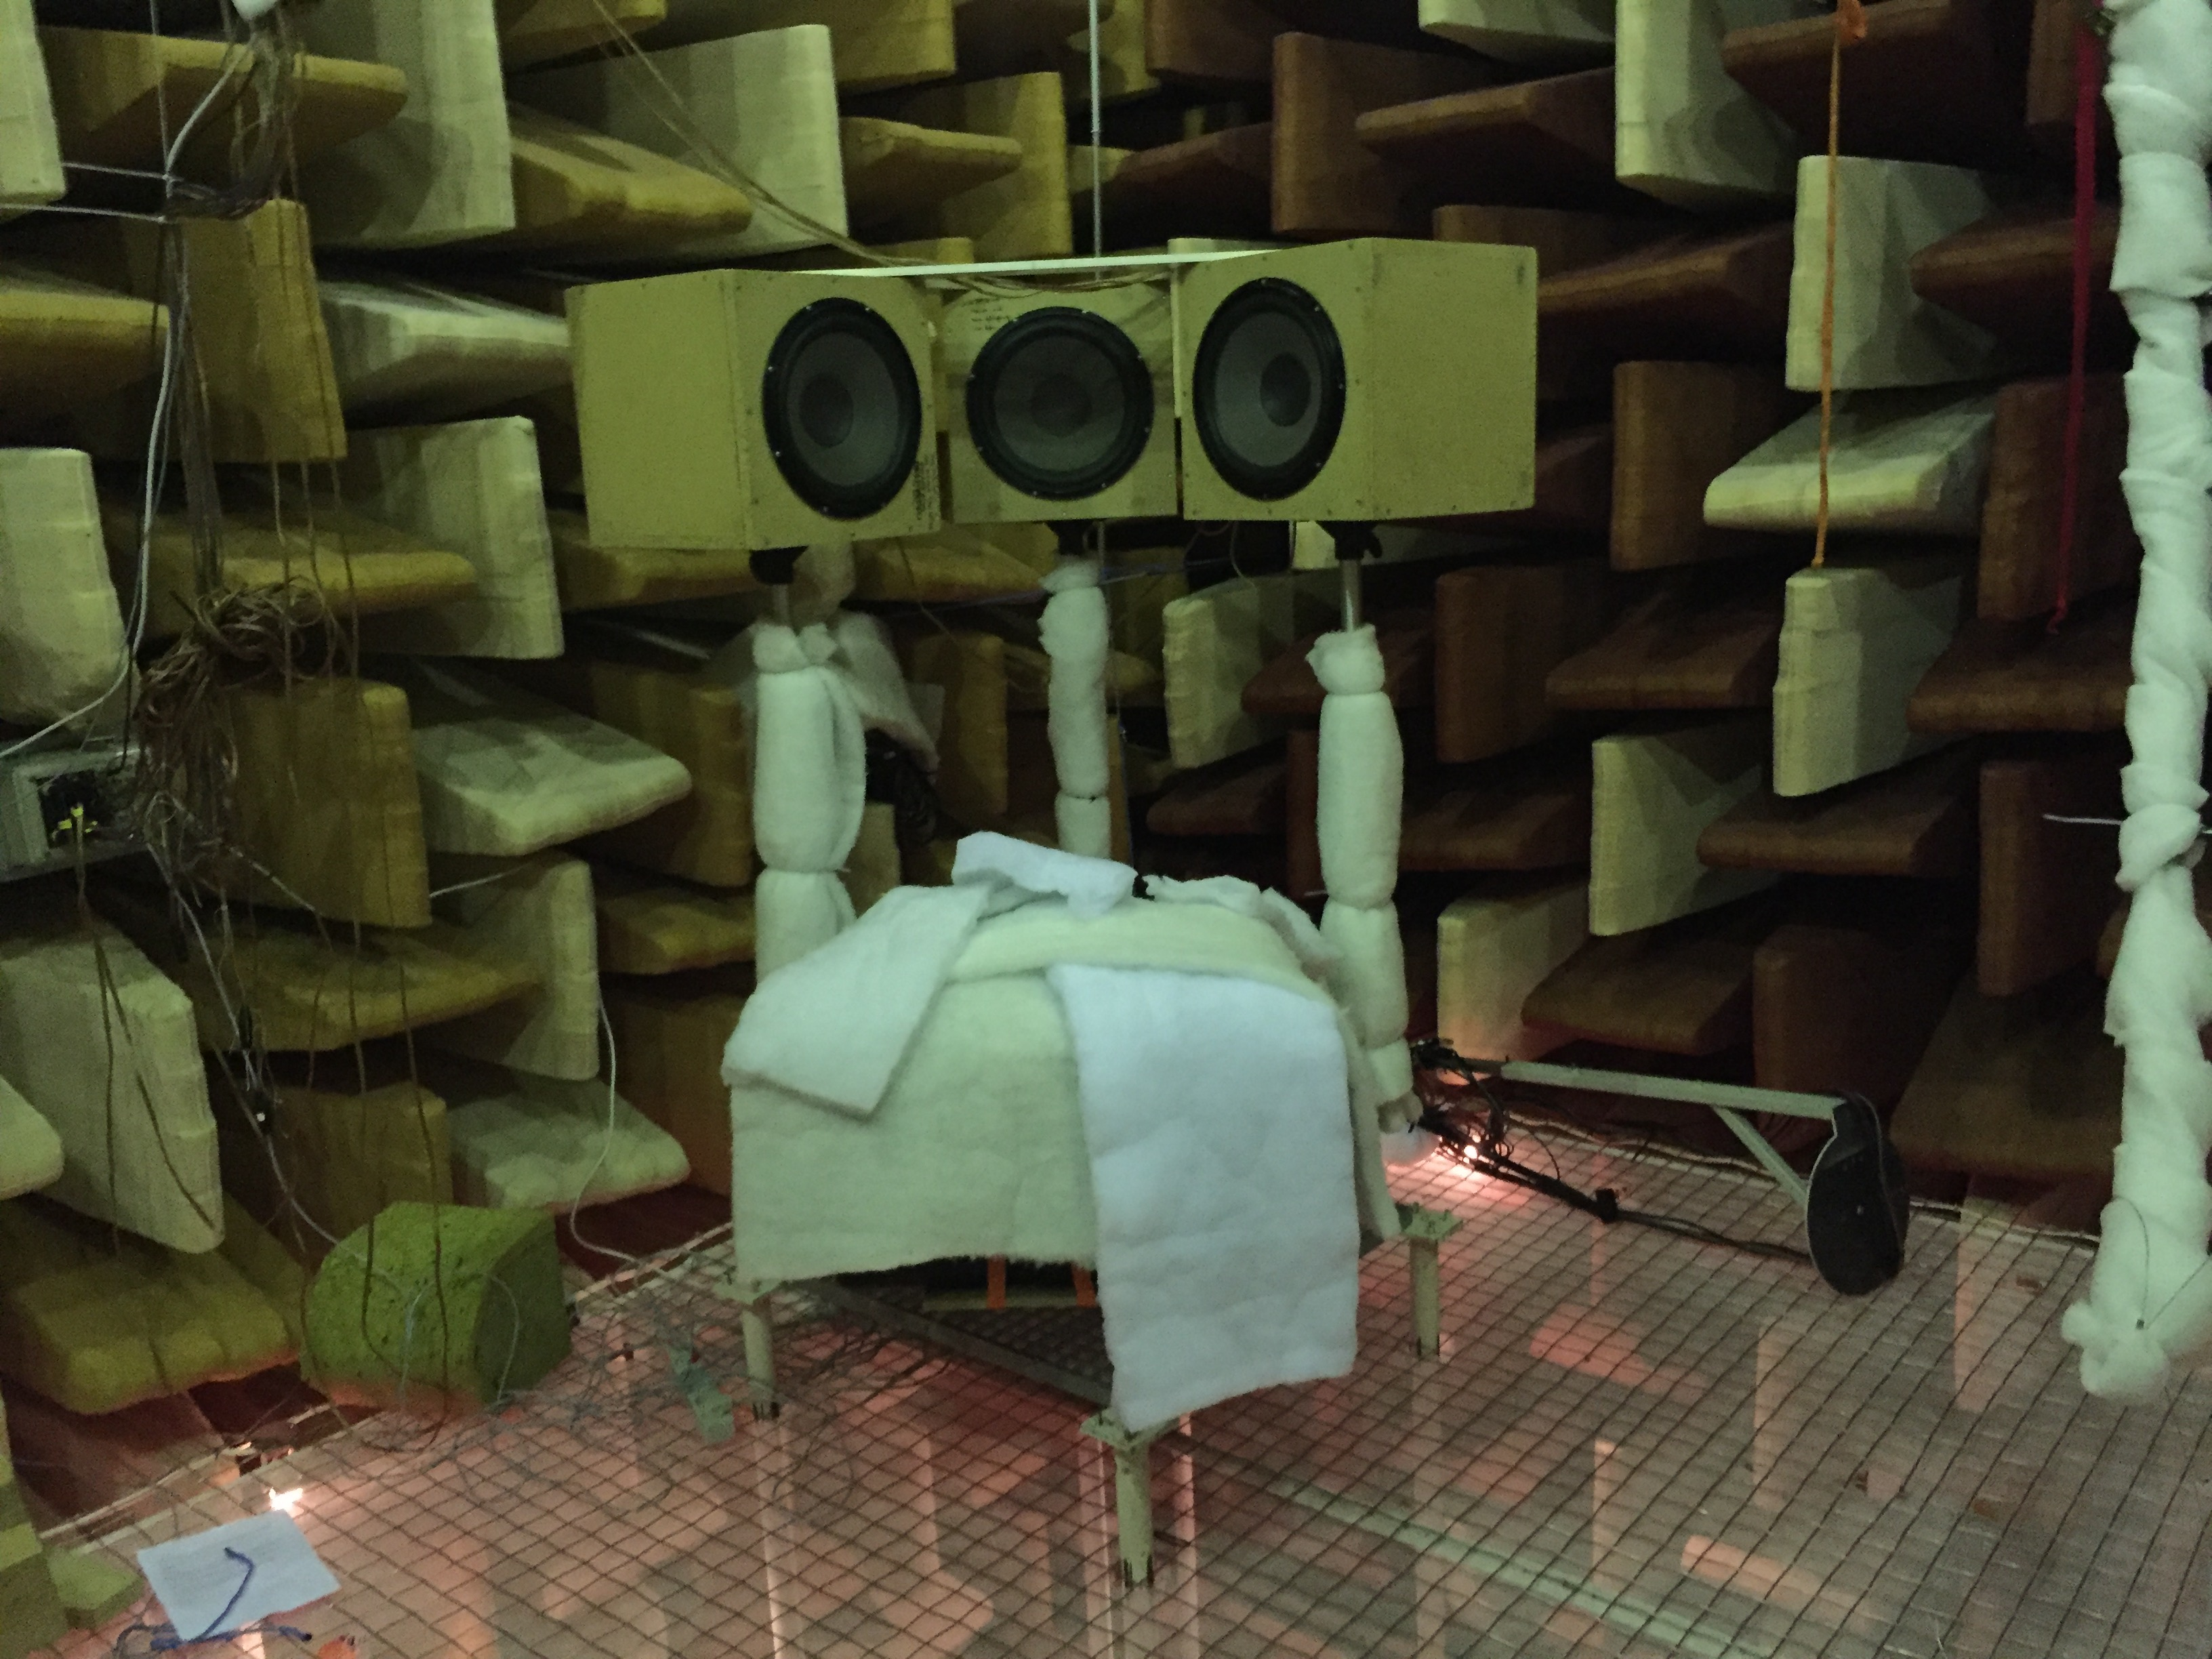
\includegraphics[width=1\textwidth]{the_setup}
	\caption{A picture of the final setup in the anechoic chamber at \gls{aau}}
		\label{fig:the_setup}
\end{figure}

The rigidity of the speaker stand construction is insufficient to keep the loudspeakers in precise positions relative to eachother. Therefore a triangular wooden piece is added, connection the top sides of all the loudspeakers. The construction tends to oscillate for a time of roughly \SI{2}{\second} after the turntable stops rotating, before the loudspeaker settle. With addition of the top wood plate, the position of the speakers sufficiently precise. However, the adding the top plate also leads to another parameter, that has to be adjusted before measurements, in order to ensure, that the main axis of the speakers is on the horizontal plane. 
The top plate is shown in \autoref{fig:array_pic}. The figure also gives an impression about the spacing and sizes of the speaker cabinets.

\begin{figure}[H]
	\centering
    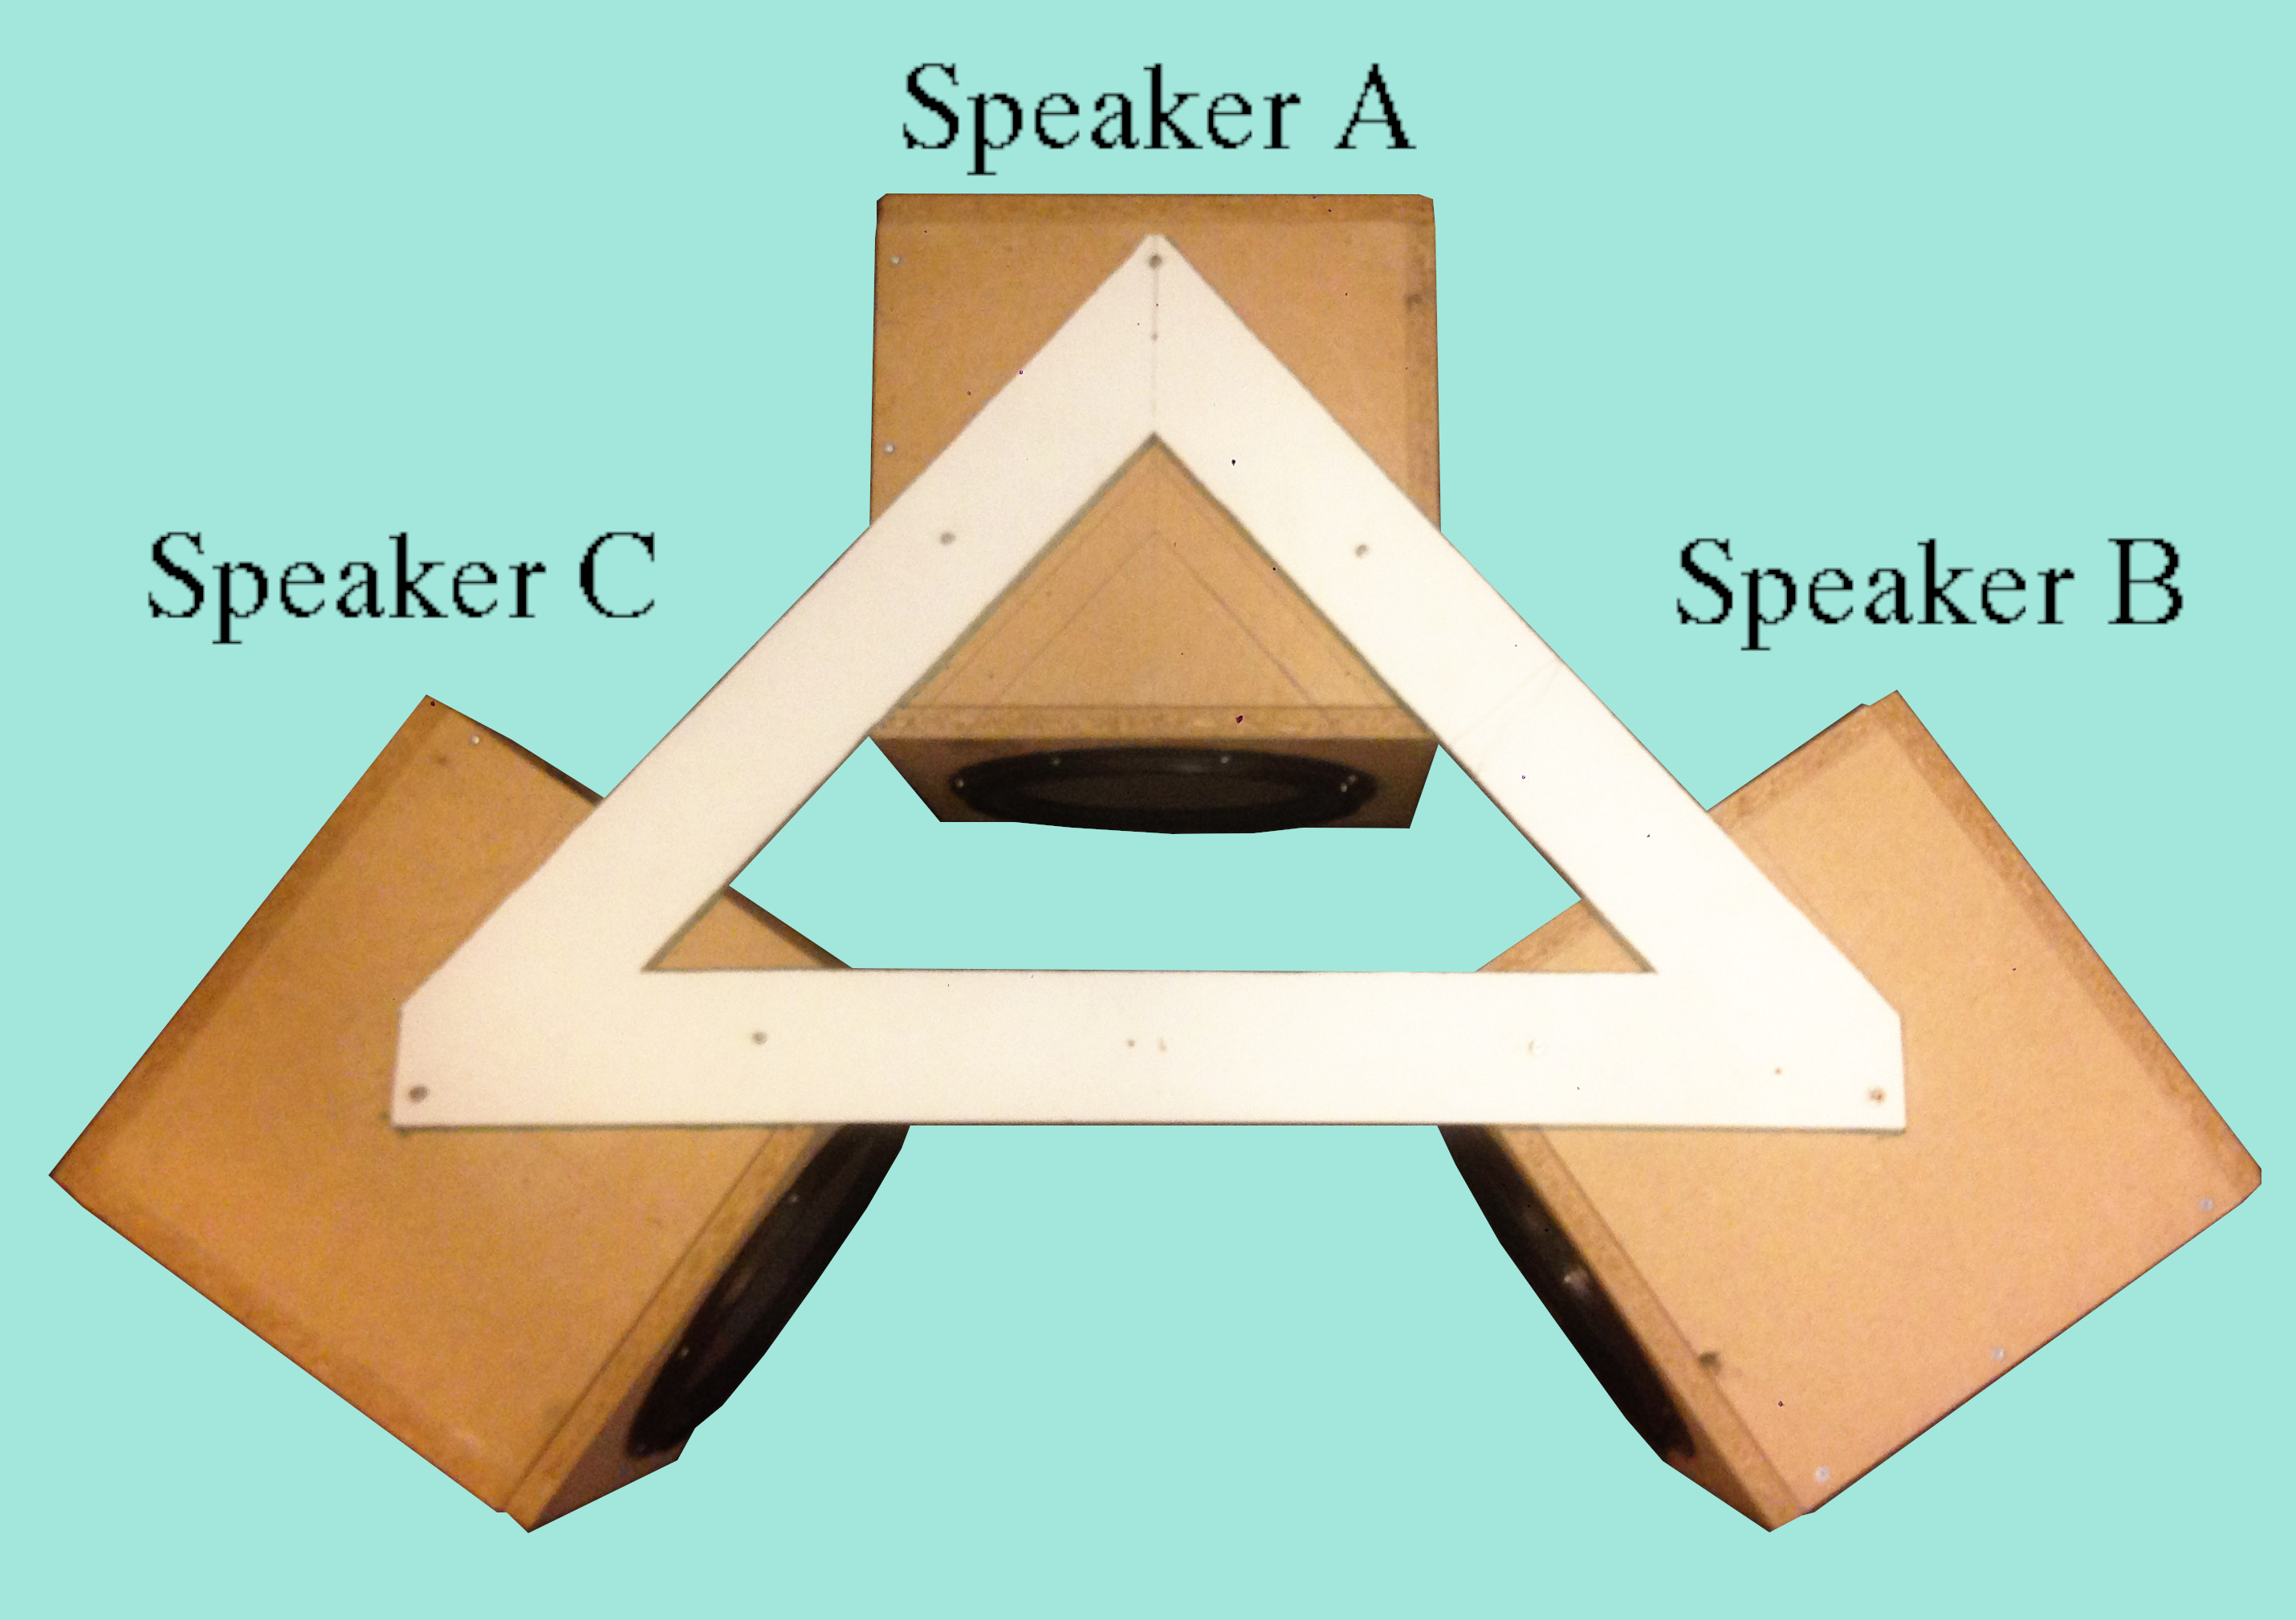
\includegraphics[width=1\textwidth]{speaker_array.jpg}
    \caption{Speaker array arrangement}
    \label{fig:array_pic}
\end{figure}





